\chapter{Arquitectura del Sistema}
\label{cap:descripcionTrabajo}


\section{Diagramas de clases}
Para facilitar la comprensión de la herramienta, se han realizado unos diagramas de clases que describen la arquitectura del sistema.\\

\begin{figure}[]
	\centering
	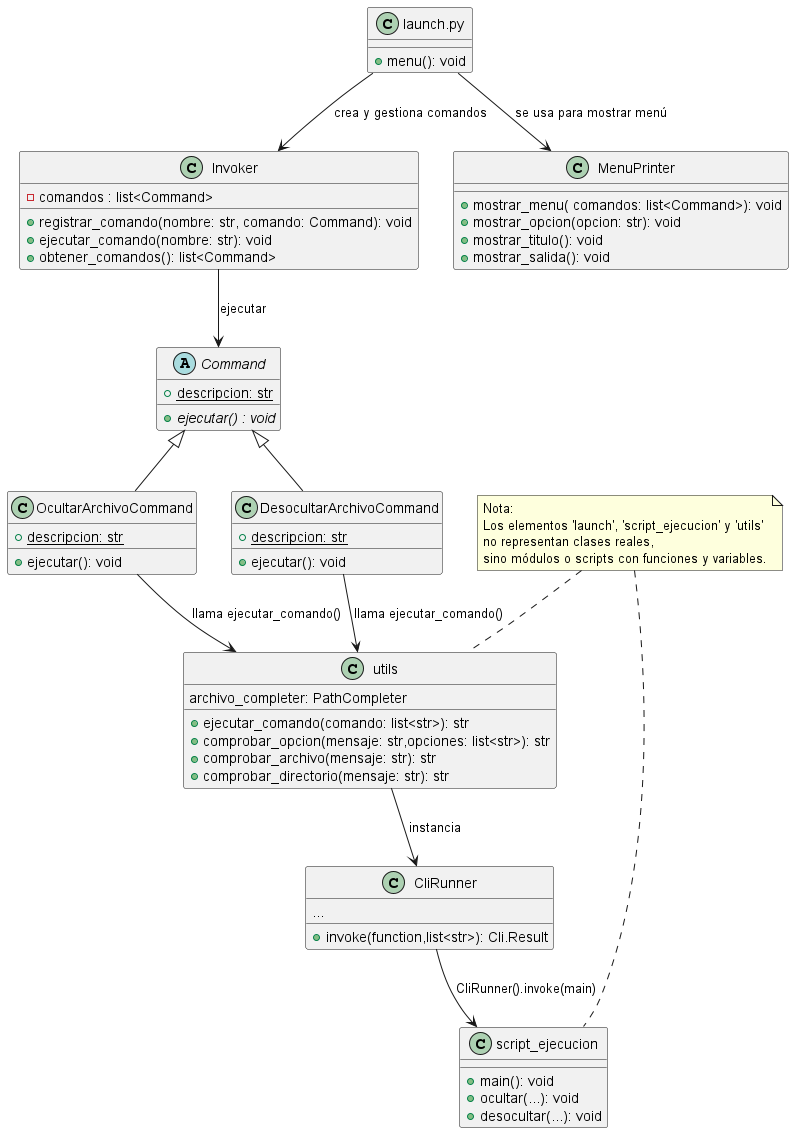
\includegraphics[width = 1 \textwidth]{Imagenes/Diagramas/clases/Diagrama_Launcher_Invoker_Comandos.png}
	\caption[Diagrama de clases CLI.]{Diagrama de clases: CLI. Elaboración propia.}
	\label{fig:Launch}
    \end{figure}

La interacción con el usuario se inicia en el \textit{launch}, donde se instancian tanto el \textit{Invoker} como el \textit{MenuPrinter}, quienes son respectivamente los responsables de gestionar los comandos e imprimir por consola las opciones principales del programa. Los comandos son registrados y ejecutados por el \textit{Invoker}, estos extienden de una clase abstracta denominada \textit{Command}. Gracias a esta estructura, la creación de comandos es más sencilla en caso de que se desee ampliar la funcionalidad del sistema. Posteriormente, los comandos son ejecutados creando la instrucción correspondiente que será enviada al script de ejecución mediante utils, esta instrucción se genera según las opciones indicadas al comando, figura \ref{fig:Launch}.\\


\begin{figure}[]
	\centering
	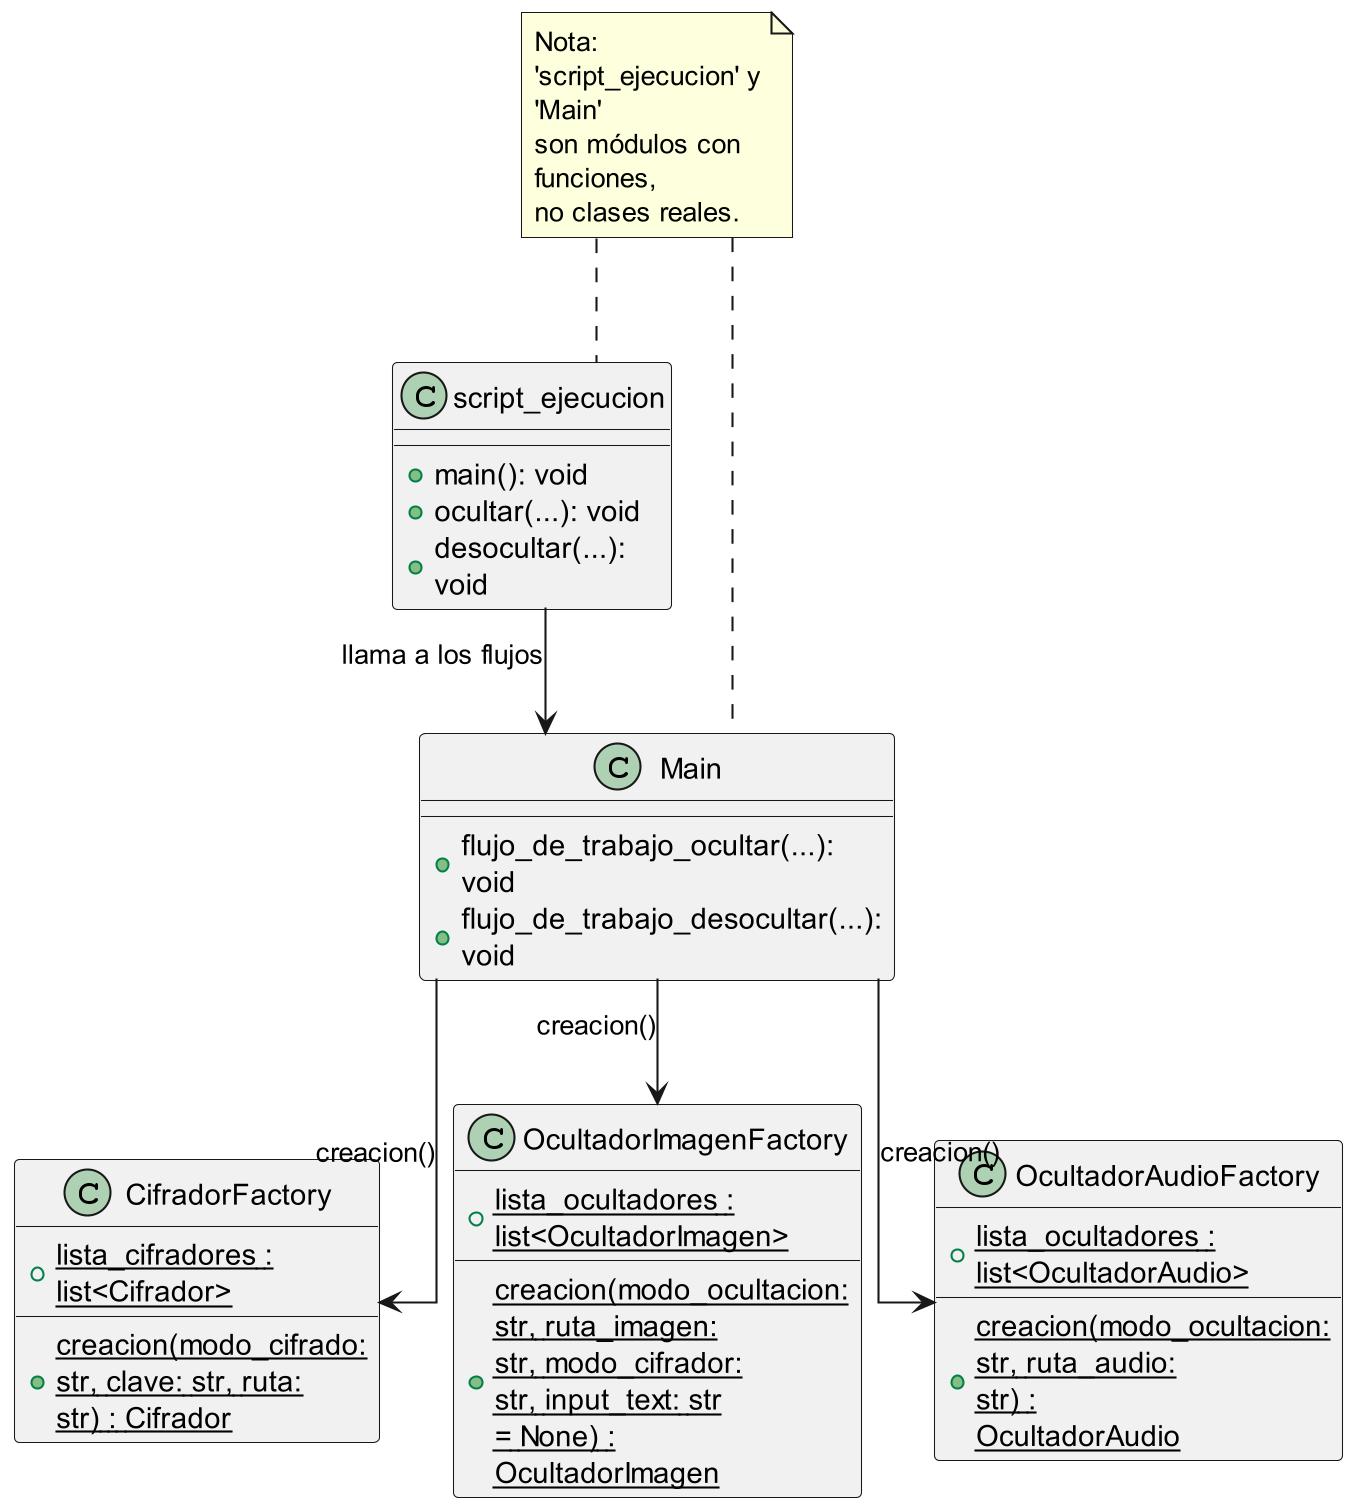
\includegraphics[width = 1 \textwidth]{Imagenes/Diagramas/clases/Diagrama_07_ScriptEjecucion_FlujoCompleto.png}
	\caption[Diagrama de clases: Main.]{Diagrama de clases: Main. Elaboración propia.}
	\label{fig:scrip_main}
\end{figure}


A continuación, figura \ref{fig:scrip_main}, el método correspondiente del main se invoca a  través del script con todas las opciones seleccionadas como argumentos. Seguidamente, las instancias concretas de cifrado y ocultación se crean mediante los \textit{Factories} y cada instancia se llama para que ejecute su función correspondiente.\\


\begin{figure}[]
	\centering
	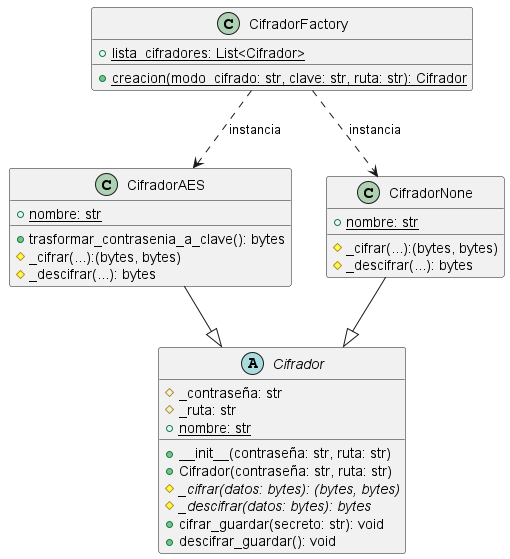
\includegraphics[width = 0.7 \textwidth]{Imagenes/Diagramas/clases/Diagrama_Cifradores.png}
	\caption[Diagrama de clases: Cifradores.]{Diagrama de clases: Cifradores. Elaboración propia.}
	\label{fig:cifradores}
\end{figure}


En la figura \ref{fig:cifradores} se puede observar la clase abstracta Cifrador que se extiende por 2 cifradores concretos, que se instancian mediante el \textit{Factory} correspondiente en función de las opciones que se han seleccionado de cifrado y descifrado. \\

Se puede elegir entre dos cifradores, \textit{none}, el cual no cifra, y AES, el cual cifra los datos utilizando el algoritmo AES en modo CBC. Antes de que se cifre el mensaje, se verifica que los datos tengan un tamaño múltiplo del tamaño del bloque y se crea la clave transformando la contraseña en una clave de 16 bytes utilizando SHA256\footnote{\cite{NISTFIPS1804}.} y truncando el \textit{hash} al tamaño necesario. El proceso de descifrado consiste en transformar la contraseña a clave como en el cifrado y con ella se descifraría el mensaje.\\

Los ocultadores tanto en imágenes como en audio siguen el mismo diseño que los cifradores, como se puede comprobar en las figuras \ref{fig:ocultadorimg} y \ref{fig:ocultadoraudio}. Este diseño está orientado a la escalabilidad, facilitando la incorporación de nuevas funcionalidades.\\

En los ocultadores en imagen se dispone de ocultación mediante LSB o \textit{Text}.\\
Con la ocultación LSB, primero se calcula el tamaño de los datos a ocultar en binario para indicarlo en una cabecera de 32 bits \footnote{Se opta por usar 32 bits, que pueden representar hasta archivos de 512MB aproximadamente, en lugar de valores ligeramente menores pero mas ajustados a los posibles tamaños de los archivos que se manejan, porque la diferencia en capacidad es marginal y, de este modo, se evitan posibles problemas al manejar imágenes y, sobre todo, audios de gran tamaño.} que serán los 32 primeros datos que se ocultarán en la imagen. Después, se comprueba que la imagen tiene suficiente espacio para ocultar el mensaje completo, el cual consiste en los 32 bits de la cabecera más el número de bits de datos a ocultar, y se van recorriendo los píxeles de la imagen añadiendo en el bit menos significativo de cada píxel un bit del mensaje hasta que esté completamente oculto. El tamaño mínimo de la imagen tiene que ser:\\
\[
\text{MB mínimos de imagen} = \frac{\left( \frac{T + M}{3} \right) \times 3}{1024^2} = \frac{T + M}{1024^2}
\]
\[
\noindent\text{donde } T = \text{tamaño de la cabecera en bits} \text{ y } M = \text{tamaño del secreto en bits.}
\]



En el proceso de desocultación, primero se leen los 32 primeros bits menos significativos para obtener el tamaño del mensaje que se va a leer y, posteriormente, se lee el mensaje completo. \\

Con la ocultación \textit{Text}, si los datos vienen cifrados se codifican en base64 antes de que se escriban, si no están cifrados se escriben tal cual. Esto se debe a que al cifrar la información, los caracteres imprimibles pueden haberse convertido en no imprimibles. Primero, se carga el archivo ``configuracion.toml'', archivo de configuración que, entre otras cosas, contiene la información del tamaño de la fuente, la anchura máxima y la ruta de la fuente que se va a usar. Posteriormente, se calcula la  anchura máxima de las líneas y se procede a insertar el mensaje en una lista de listas de caracteres, siendo cada lista una línea del texto que se cargará en la imagen. Por último, se crea la imagen, con un tamaño fijo si se va a usar SSTV o con el tamaño necesario si no, y se dibuja el texto en ella.\\ 

Para desocultar se utilizan dos motores OCR (\textit{Optical Character Recognition}) que extraen el texto de la imagen. Se han usado dos debido a que uno está diseñado para reconocer palabras completas, en caso de no cifrado de datos, y el otro para reconocer caracteres sueltos, caso de cifrado y codificación en base64. \\

En los ocultadores en audio se dispone de ocultación mediante LSB o SSTV.\\
Con la ocultación LSB, el procedimiento sería el mismo que la ocultación en la imagen LSB, pero esta vez se ocultará en los \textit{frames} del audio y no en píxeles. El descifrado sería también equivalente. El tamaño mínimo del audio tiene que ser:\\ 
\[
\text{MB mínimos de audio} = \frac{T + I + E}{1024^2}
\]
\[
\begin{aligned}
\text{donde } T &= \text{tamaño de la cabecera en bits}, \\
I &= \text{tamaño de la imagen en bits}, \\
E &= \text{encabezado de WAV en bits.}
\end{aligned}
\]


Con la ocultación SSTV, se lee y se redimensiona la imagen a ocultar con \textit{Pillow} y se modula la imagen en una señal SSTV usando el modo SSTV seleccionado, para los cuales es necesario que la imagen transmitida tenga un tamaño fijo. En cambio, para desocultar, se abre QSSTV\footnote{Https://www.cqsstv.com/ .} y, dependiendo de si se ha seleccionado el modo streaming o no, se muestra por terminal la ruta del archivo que debe seleccionar para decodificar en QSSTV y dónde se debe guardar para seguir con el correcto funcionamiento de la herramienta.\\

Las tres \textit{Factories} mencionadas se han  implementado como subclases que extienden de una \textit{factory} abstracta denominada \textit{AbstractFactory}, tal como se ve en la figura \ref{fig:factories}. Como hemos visto antes, esto también es una facilidad en caso de que se quieran incorporar nuevos medios en los que ocultar información.\\

\begin{figure}[h]
	\centering
	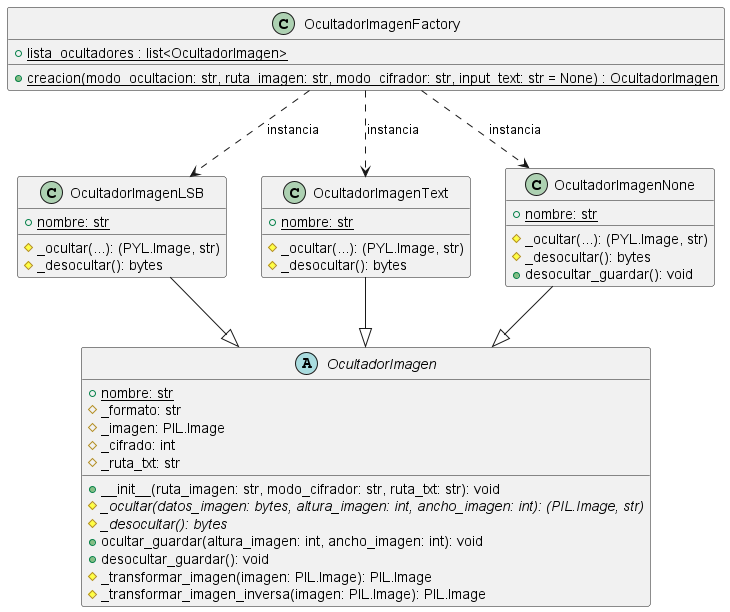
\includegraphics[width = 0.9 \textwidth]{Imagenes/Diagramas/clases/Diagrama_Ocultadores_Completo.png}
	\caption[Diagrama de clases: Ocultadores en imagen.]{Diagrama de clases: Ocultadores en imagen. Elaboración propia.}
	\label{fig:ocultadorimg}
\end{figure}


\begin{figure}[]
	\centering
	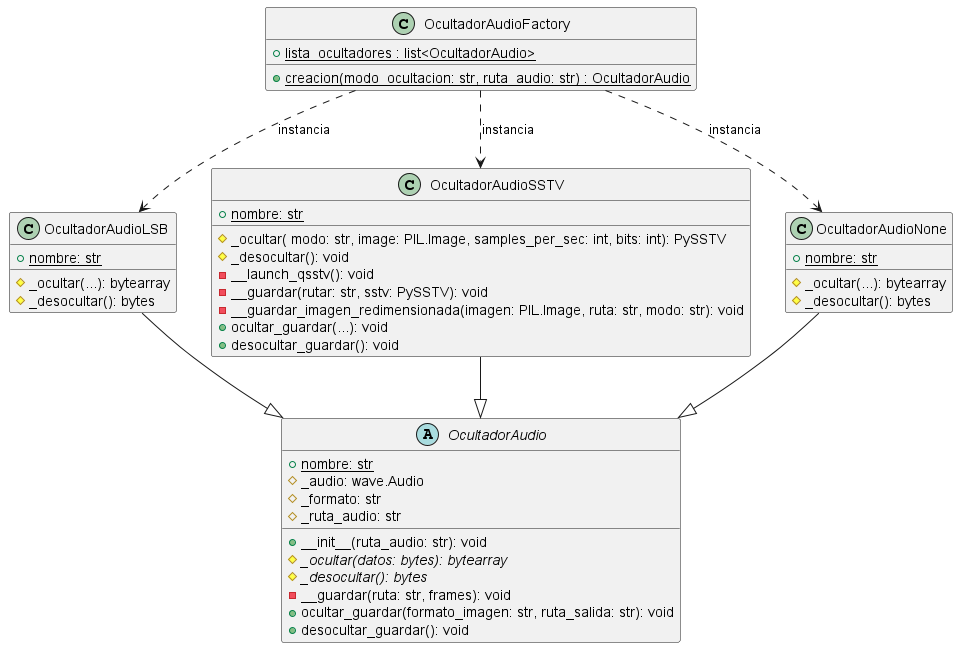
\includegraphics[width = 1 \textwidth]{Imagenes/Diagramas/clases/Diagrama_Ocultadores_Audio_Sin_AbstractFactory.png}
	\caption[Diagrama de clases: Ocultadores en audio.]{Diagrama de clases: Ocultadores en audio. Elaboración propia.}
	\label{fig:ocultadoraudio}
\end{figure}




\begin{figure}[]
	\centering
	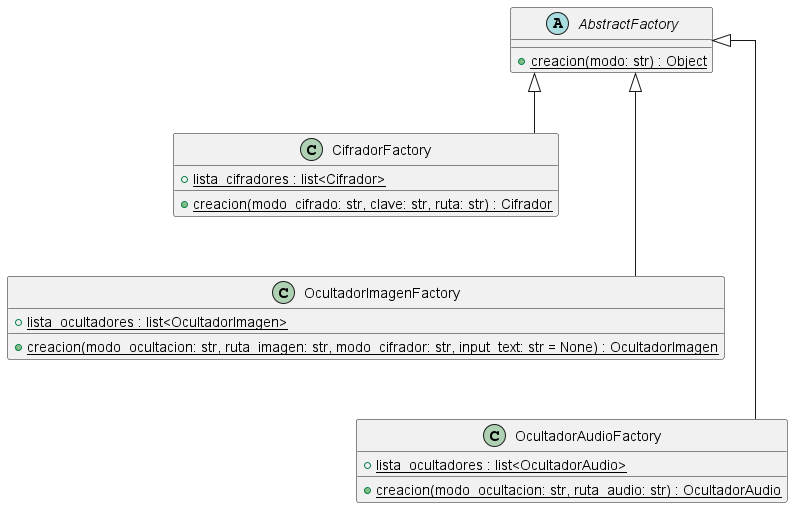
\includegraphics[width = 1.0 \textwidth]{Imagenes/Diagramas/clases/Diagrama_AbstractFactory_Horizontal.png}
	\caption[Diagrama de clases: Fábricas.]{Diagrama de clases: Fábricas. Elaboración propia.}
	\label{fig:factories}
\end{figure}
\FloatBarrier

\section{Diagramas de secuencia}
A continuación, se describirán los diagramas de secuencia en los que se reflejan los flujos de ejecución del programa.\\
\begin{figure}[h]
	\centering
	\includegraphics[width = 0.85 \textwidth]{Imagenes/Diagramas/Ini.png}
	\caption[Diagrama de secuencia: \textit{Launch} parte 1.]{Diagrama de secuencia: \textit{Launch} parte 1. Elaboración propia.}
	\label{fig:Inicio}
\end{figure}


En primer lugar, como se ve en la figura \ref{fig:Inicio}, se crean las instancias encargadas de la impresión gráfica del menú por comandos, de la ejecución del comando seleccionado y del registro de los comandos principales necesarios. A continuación, se crean las instancias de cada comando y se registran en el invocador.



\begin{figure}[h]
	\centering
	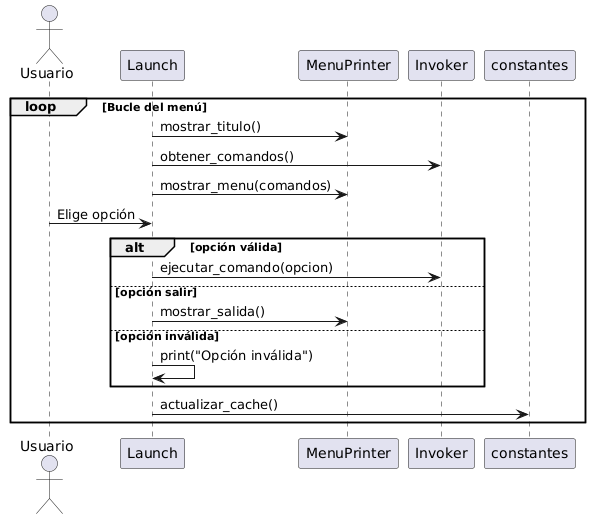
\includegraphics[width = 0.7 \textwidth]{Imagenes/Diagramas/Menu.png}
	\caption[Diagrama de secuencia: \textit{Launch} parte 2.]{Diagrama de secuencia: \textit{Launch} parte 2. Elaboración propia.}
	\label{fig:Menu}
\end{figure}
\FloatBarrier
En la figura \ref{fig:Menu} se ve el bucle principal del lanzador, en el cual se muestra el título del programa y las opciones de los comandos disponibles, figura \ref{fig:Titulo}. La opción elegida se valida y, posteriormente, se ejecuta. Por último, la caché se actualiza.

\begin{figure}[h]
	\centering
	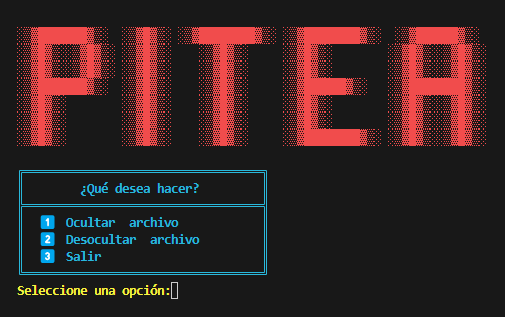
\includegraphics[width = 0.8  \textwidth]{Imagenes/Diagramas/Titulo.png}
	\caption[Menú de inicio.]{Menú de inicio. Captura de pantalla de la herramienta.}
	\label{fig:Titulo}
\end{figure}

\FloatBarrier

\begin{figure}[h]
	\centering
	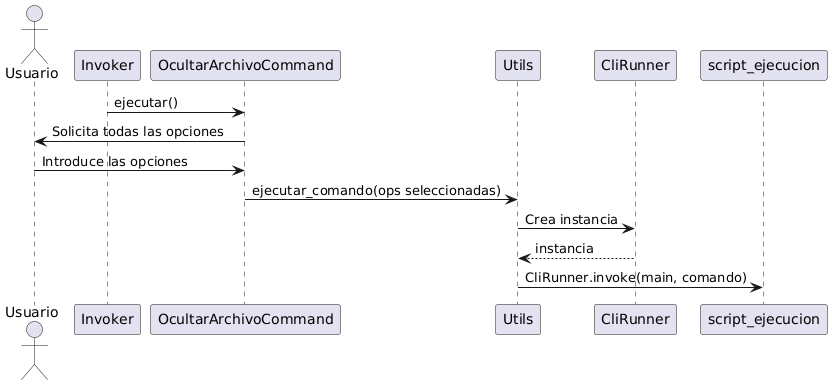
\includegraphics[width = 1  \textwidth]{Imagenes/Diagramas/ocult_cmd.png}
	\caption[Diagrama de secuencia: Comando de ocultación.]{Diagrama de secuencia: Comando de ocultación. Elaboración propia.}
	\label{fig:Oculcmd}
\end{figure}

\begin{figure}[h]
	\centering
	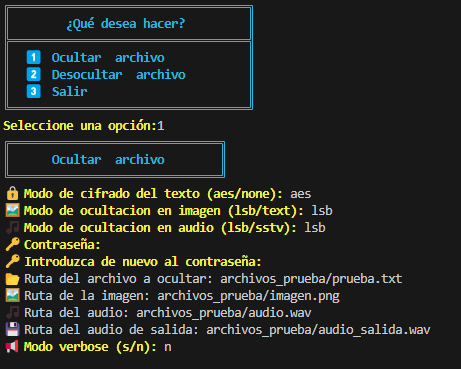
\includegraphics[width = 0.6  \textwidth]{Imagenes/Diagramas/Opciones.png}
	\caption[Opciones a rellenar por el usuario.]{Opciones a rellenar por el usuario. Captura de pantalla de la herramienta.}
	\label{fig:Opciones}
\end{figure}
\FloatBarrier
En caso de que se escoja ocultar (opción con índice 1) se invoca al método \textit{ejecutar\_comando(1)} del \textit{invoker} que se encarga de que se llame al método \textit{ejecutar()} del comando seleccionado, en este caso \textit{OcultarArchivoComamand}. El comando correspondiente muestra al usuario las opciones posibles a la hora de cifrar y ocultar el archivo, figura \ref{fig:Opciones}. Posteriormente, las opciones seleccionadas se envían al módulo \textit{utils}, mediante el cual se crea una instancia \textit{CliRunner}, con la cual se invoca el script de ejecución con las instrucciones a ejecutar, tal como se observa en la figura \ref{fig:Oculcmd}.  

\begin{figure}[h]
	\centering
	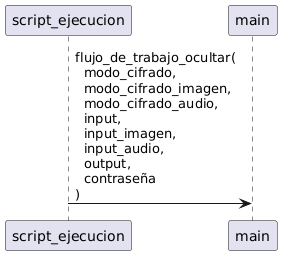
\includegraphics[width = 0.5  \textwidth]{Imagenes/Diagramas/ocul/llamada_flujo_ocul.png}
	\caption[Diagrama de secuencia: Llamada al flujo de ocultación.]{Diagrama de secuencia: Llamada al flujo de ocultación. Elaboración propia.}
	\label{fig:llmadafluocul}
\end{figure}
\FloatBarrier

Como se muestra en la figura \ref{fig:llmadafluocul}, el \textit{main} del programa se invoca desde el script de ejecución, utilizando las opciones que se seleccionaron anteriormente como argumentos.

\begin{figure}[h]
	\centering
	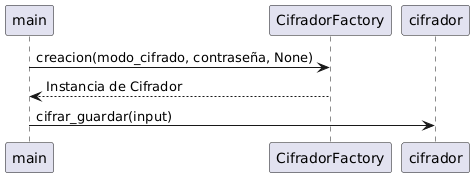
\includegraphics[width = 0.8  \textwidth]{Imagenes/Diagramas/ocul/fase_cifrado.png}
	\caption[Diagrama de secuencia: Creación del Cifrador.]{Diagrama de secuencia: Creación del Cifrador. Elaboración propia.}
	\label{fig:cifcreacion}
\end{figure}
\FloatBarrier

Ya en el main, una instancia de Cifrador se crea a través del \textit{CifradorFactory} y luego esta se invoca para que ejecute su acción, figura \ref{fig:cifcreacion}.

\begin{figure}[h]
	\centering
	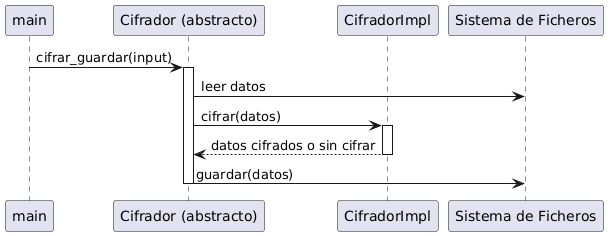
\includegraphics[width = 0.8  \textwidth]{Imagenes/Diagramas/ocul/cifrador.png}
	\caption[Diagrama de secuencia: Cifrado de los datos.]{Diagrama de secuencia: Cifrado de los datos. Elaboración propia.}
	\label{fig:cifrado}
\end{figure}
\FloatBarrier

Primero en el Cifrador abstracto, se leen los datos desde el sistema de ficheros, luego estos se cifran en el Cifrador concreto seleccionado y, por último, se guardan de nuevo, tal como se representa en la figura \ref{fig:cifrado}.  

\begin{figure}[h]
	\centering
	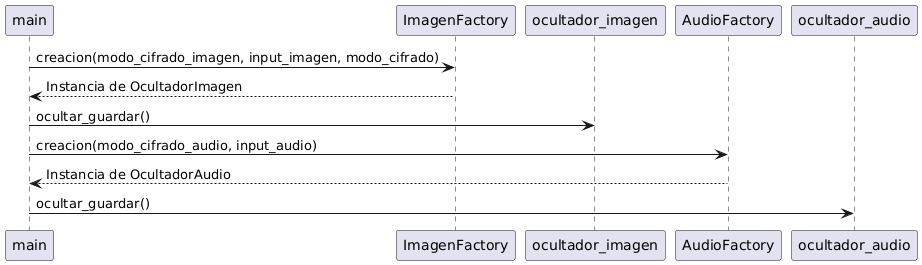
\includegraphics[width = 1  \textwidth]{Imagenes/Diagramas/ocul/fase_ocul.png}
	\caption[Diagrama de secuencia: Creación de los ocultadores.]{Diagrama de secuencia: Creación de los ocultadores. Elaboración propia.}
	\label{fig:ocultacion}
\end{figure}
\FloatBarrier

A continuación, en la figura \ref{fig:ocultacion}, una vez que los datos han sido cifrados, se crean instancias de los ocultadores en orden. En primer lugar, se instancia el ocultador en imágenes seguido del ocultador en audio.  Tras cada instanciación, se invoca el método correspondiente de cada ocultador.

\begin{figure}[h]
	\centering
	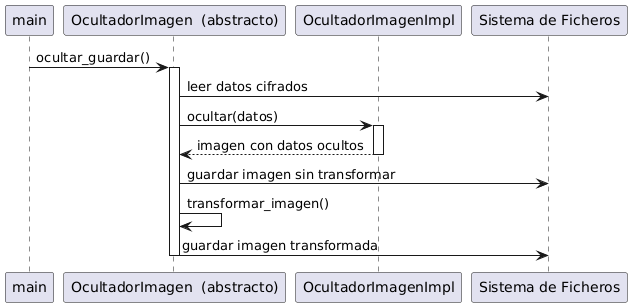
\includegraphics[width = 0.8  \textwidth]{Imagenes/Diagramas/ocul/oculimg.png}
	\caption[Diagrama de secuencia: Ocultación en la imagen.]{Diagrama de secuencia: Ocultación en la imagen. Elaboración propia.}
	\label{fig:oculimg}
\end{figure}
\FloatBarrier

Cuando se invoca el \textit{ocultar\_guardar()} del ocultador en imagen, como se puede ver en la figura \ref{fig:oculimg}, se leen los datos cifrados y se ocultan en la imagen. Posteriormente, se almacena la imagen con los datos ocultos, se le aplica una transformada para dificultar la identificación del orden de los datos ocultos y, por último, se guarda nuevamente.\\

En la figura \ref{fig:transformacion2} podemos ver cómo las imágenes son transformadas. La transformada que se usa consiste en dividir la imagen en 4 partes, reordenar estas 4 partes y sobre la nueva imagen se hace una negación bit a bit, lo que genera que visualmente los colores se inviertan. En el ejemplo de la figura \ref{fig:transformacion1} se puede observar que, si se escoge una imagen sin un patrón significativo, no se puede saber desde la imagen transformada cómo es la original, imposibilitando saber tanto los valores originales de los píxeles como el orden correcto de las partes de la imagen.

\begin{figure}[h]
	\centering
	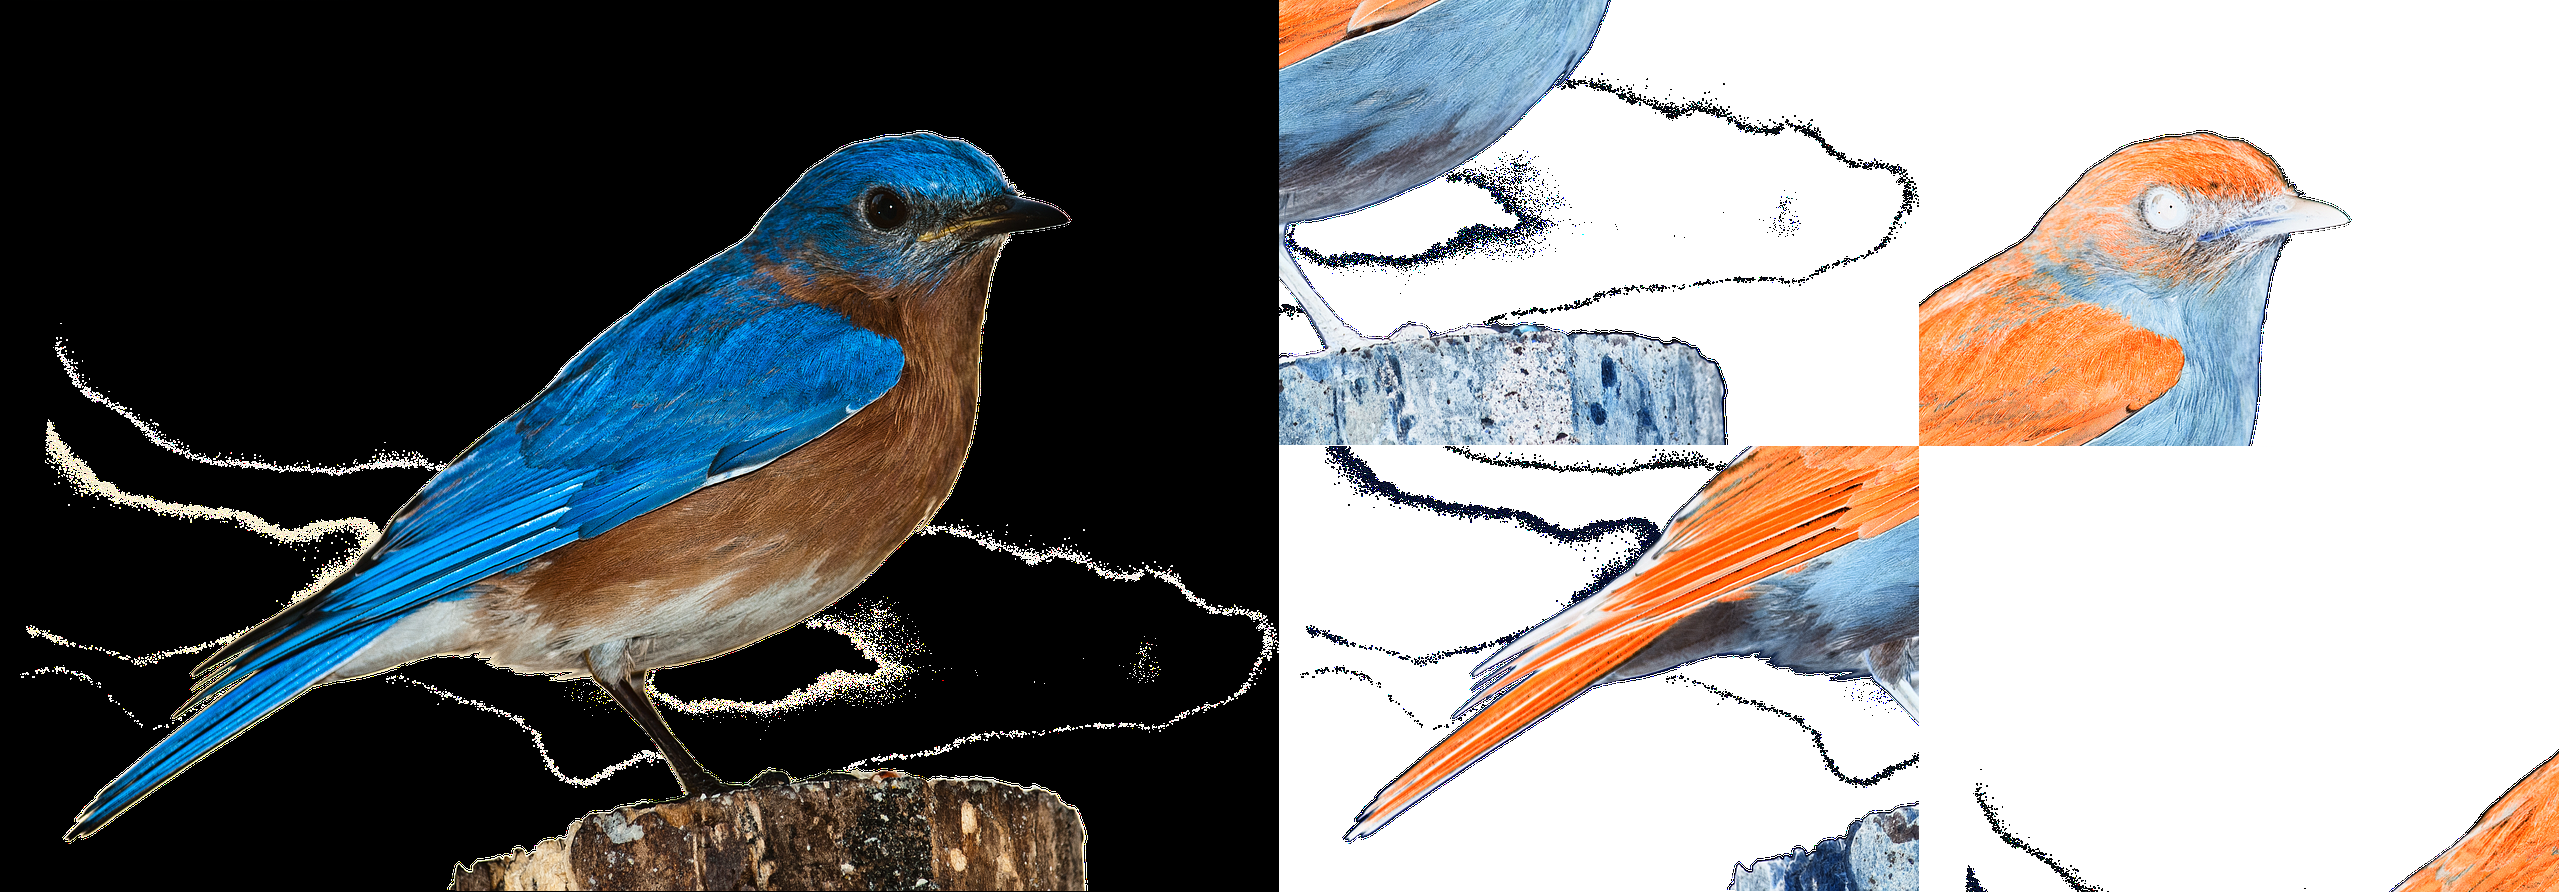
\includegraphics[width = 0.45  \textwidth]{Imagenes/prueba_campo2_2/transformacion.png}
	\caption[Imagen con ocultación por LSB transformada.]{Imagen con ocultación por LSB antes y después de ser transformada. Elaboración propia.}
	\label{fig:transformacion2}
\end{figure}

\begin{figure}[h]
	\centering
	
\includegraphics[width = 0.45 \textwidth]{Imagenes/Diagramas/trasnfromada2.png}
	\caption[Imagen con ocultación por LSB transformada.]{Imagen con ocultación por LSB antes y después de ser transformada. Elaboración propia.}
	\label{fig:transformacion1}
\end{figure}


\FloatBarrier

\begin{figure}[h]
	\centering
	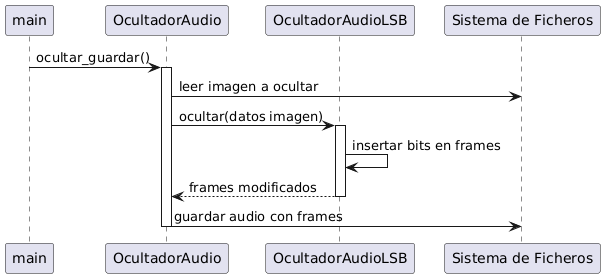
\includegraphics[width = 0.8  \textwidth]{Imagenes/Diagramas/ocul/audiolsb.png}
	\caption[Diagrama de secuencia: Ocultación en un audio mediante técnica LSB.]{Diagrama de secuencia: Ocultación en un audio mediante técnica LSB. Elaboración propia.}
	\label{fig:audiolsb}
\end{figure}
\FloatBarrier

En caso de querer ocultar en un audio mediante LSB, primero, la imagen con los datos ocultos que fue transformada se lee desde el sistema de ficheros, después se oculta en los frames del audio, y por último, se guarda el audio con datos ocultos, figura \ref{fig:audiolsb}.

\begin{figure}[h]
	\centering
	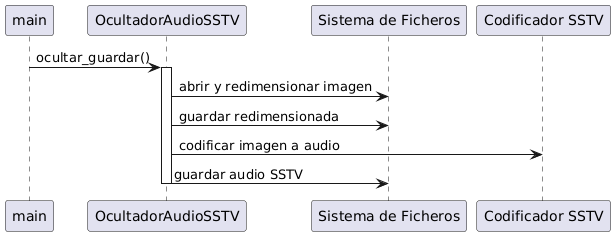
\includegraphics[width = 0.8  \textwidth]{Imagenes/Diagramas/ocul/audiosstv.png}
	\caption[Diagrama de secuencia: Modulación SSTV de la imagen.]{Diagrama de secuencia: Modulación SSTV de la imagen. Elaboración propia.}
	\label{fig:audiosstv}
\end{figure}
\FloatBarrier

En caso de querer generar una señal SSTV, primero se lee la imagen desde el sistema de ficheros, se redimensiona y,  posteriormente, se guarda. A continuación, esta imagen se modula en una señal de audio SSTV, la cual se guarda en el sistema de ficheros nuevamente, tal como se representa en la figura \ref{fig:audiosstv}.

\begin{figure}[h]
	\centering
	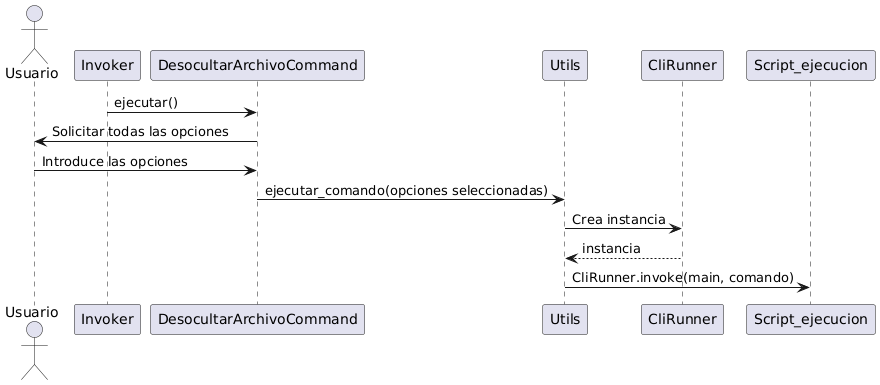
\includegraphics[width = 1  \textwidth]{Imagenes/Diagramas/desocul/desoculcmd.png}
	\caption[Diagrama de secuencia: Comando de desocultación.]{Diagrama de secuencia: Comando de desocultación. Elaboración propia.}
	\label{fig:desoculcmd}
\end{figure}
\FloatBarrier

En caso de que se escoja desocultar (opción con índice 2) se invoca al método \textit{ejecutar\_comando(2)} del \textit{invoker} que se encarga de que se llame al método \textit{ejecutar()} del comando seleccionado, en este caso \textit{DesocultarArchivoCommand}, en el que se solicitan las opciones de desocultación al usuario. Posteriormente, las opciones seleccionadas se envían al módulo \textit{utils}, mediante el cual se crea una instancia \textit{CliRunner}, con la cual se invoca el script de ejecución con las instrucciones a ejecutar.

\begin{figure}[h]
	\centering
	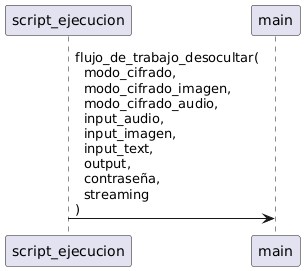
\includegraphics[width = 0.5  \textwidth]{Imagenes/Diagramas/desocul/desol.png}
	\caption[Diagrama de secuencia: Llamada al flujo de desocultación.]{Diagrama de secuencia: Llamada al flujo de desocultación. Elaboración propia.}
	\label{fig:desol}
\end{figure}
\FloatBarrier

Como se muestra en la figura \ref{fig:desol}, el main del programa se invoca desde el script de ejecución, utilizando los datos de desocultación necesarios como argumentos.


\begin{figure}[h]
	\centering
	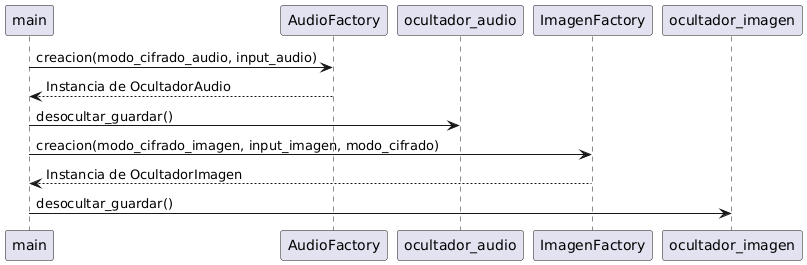
\includegraphics[width = 1  \textwidth]{Imagenes/Diagramas/desocul/fase_desocultar.png}
	\caption[Diagrama de secuencia: Creación de los ocultadores.]{Diagrama de secuencia: Creación de los ocultadores. Elaboración propia.}
	\label{fig:fase_desocultar}
\end{figure}
\FloatBarrier

En la figura \ref{fig:fase_desocultar} se puede ver que las instancias de los desocultadores se  crean en orden, primero se crea la instancia del ocultador en audio y se extrae la imagen del audio, y a continuación, la instancia del ocultador en imagen y se extrae el mensaje de la imagen.

\begin{figure}[h]
	\centering
	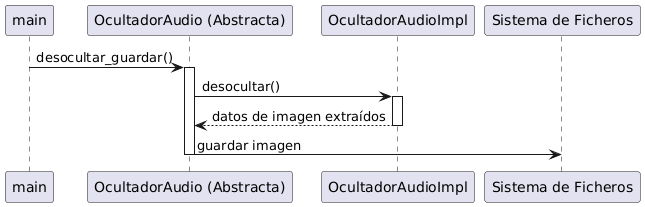
\includegraphics[width = 1  \textwidth]{Imagenes/Diagramas/desocul/desocultarlsb.png}
	\caption[Diagrama de secuencia: Desocultación de una imagen mediante LSB. ]{Diagrama de secuencia: Desocultación de una imagen en audio mediante técnica LSB. Elaboración propia.}
	\label{fig:desocultarlsb}
\end{figure}
\FloatBarrier

Primero, se invoca al ocultador abstracto, el cual se encarga de invocar al desocultador concreto, por medio de este, el flujo de audio se lee y la imagen oculta se extrae y se almacena en el sistema de ficheros, tal como se observa en la figura \ref{fig:desocultarlsb}.

\begin{figure}[h]
	\centering
	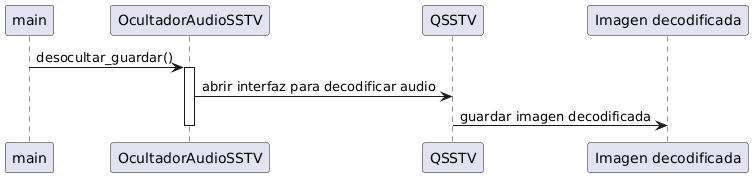
\includegraphics[width = 1  \textwidth]{Imagenes/Diagramas/desocul/desocultarsstv.png}
	\caption[Diagrama de secuencia: Decodificación del audio SSTV.]{Diagrama de secuencia: Decodificación del audio SSTV. Elaboración propia.}
	\label{fig:desocultarsstv}
\end{figure}
\FloatBarrier

En caso de tratarse de un audio SSTV, se invoca el QSSTV y una serie de pasos se indican en la terminal dependiendo de si se seleccionó el modo streaming o no, figura \ref{fig:menusstv}. Posteriormente, la imagen extraída se guarda en el sistema de ficheros, figura \ref{fig:desocultarsstv}. 

\begin{figure}[h]
	\centering
	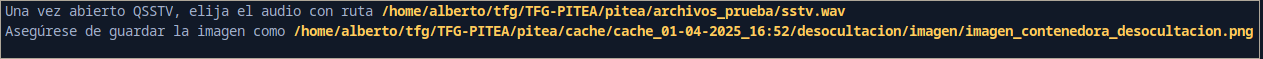
\includegraphics[width = 1  \textwidth]{Imagenes/pitea/sstv_inst.png}
	\caption[Pasos de decodificación SSTV.]{Pasos de decodificación SSTV. Captura de pantalla de la herramienta.}
	\label{fig:menusstv}
\end{figure}
\FloatBarrier

\begin{figure}[h]
	\centering
	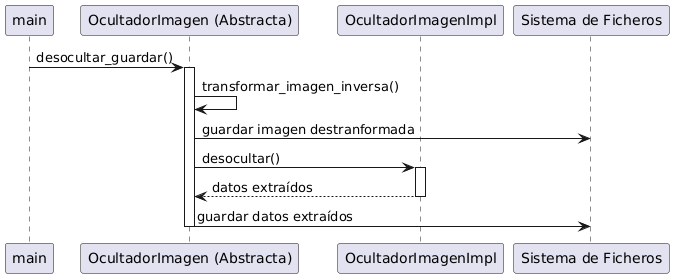
\includegraphics[width = 0.9  \textwidth]{Imagenes/Diagramas/desocul/desoculimg.png}
	\caption[Diagrama de secuencia: Recuperación del mensaje oculto en la imagen.]{Diagrama de secuencia: Recuperación del mensaje oculto en la imagen. Elaboración propia.}
	\label{fig:desoculimg}
\end{figure}
\FloatBarrier

A continuación, en el ocultador de imagen abstracto, se realiza la transformada inversa a la imagen  para recuperar el orden original de los bytes y los valores correctos de los píxeles. Una vez se realizada la transformada inversa, la imagen se guarda y el método desocultar del ocultador concreto se invoca para que los datos sean extraídos de la imagen, estos se guardan en el sistema de ficheros.

\begin{figure}[h]
	\centering
	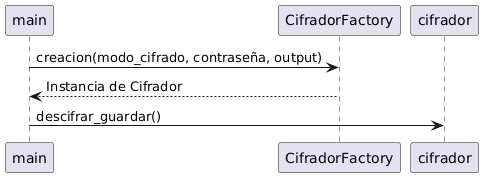
\includegraphics[width = 0.8  \textwidth]{Imagenes/Diagramas/desocul/descifrar_inst.png}
	\caption[Diagrama de secuencia: Creación del Cifrador.]{Diagrama de secuencia: Creación del Cifrador. Elaboración propia.}
	\label{fig:descifrar_inst}
\end{figure}
\FloatBarrier

Después de la desocultación, se crea una instancia de Cifrador para posteriormente invocar al método de descifrado, figura \ref{fig:descifrar_inst}.

\begin{figure}[h]
	\centering
	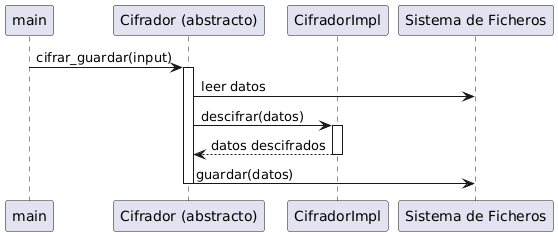
\includegraphics[width = 0.8 \textwidth]{Imagenes/Diagramas/desocul/descifrar.png}
	\caption[Diagrama de secuencia: Descifrado de los datos.]{Diagrama de secuencia: Descifrado de los datos. Elaboración propia.}
	\label{fig:descifrar}
\end{figure}
\FloatBarrier

A continuación, los datos cifrados  se leen  en el Cifrador abstracto , desde donde se invoca el proceso de descifrado del Cifrador concreto, y los datos se convierten nuevamente a texto claro. Finalmente, los datos descifrados se guardan en el sistema de ficheros.


